\documentclass[UTF8,a4paper,landscape,16pt]{paper}
\usepackage{ctex}
\usepackage{amsmath}
\usepackage{pdfpages}
\usepackage{graphicx}
\usepackage{wrapfig}
\usepackage{listings}
\usepackage{xcolor}
\usepackage{multicol}
\usepackage{float}
\usepackage{fancyhdr}
\usepackage[utf8]{inputenc}
\usepackage[landscape]{geometry}
\usepackage[figuresright]{rotating}
% Style definition file generated by highlight 3.6, http://www.andre-simon.de/ 

% Highlighting theme: Vim Editor 

\newcommand{\hlstd}[1]{\textcolor[rgb]{0,0,0}{#1}}
\newcommand{\hlnum}[1]{\textcolor[rgb]{1,0,0}{#1}}
\newcommand{\hlesc}[1]{\textcolor[rgb]{1,0.13,1}{#1}}
\newcommand{\hlstr}[1]{\textcolor[rgb]{1,0,0}{#1}}
\newcommand{\hlpps}[1]{\textcolor[rgb]{1,0,0}{#1}}
\newcommand{\hlslc}[1]{\textcolor[rgb]{0,0,1}{#1}}
\newcommand{\hlcom}[1]{\textcolor[rgb]{0,0,1}{#1}}
\newcommand{\hlppc}[1]{\textcolor[rgb]{1,0.13,1}{#1}}
\newcommand{\hlopt}[1]{\textcolor[rgb]{0,0,0}{#1}}
\newcommand{\hllin}[1]{\textcolor[rgb]{0,0,1}{#1}}
\newcommand{\hlkwa}[1]{\textcolor[rgb]{0.7,0.41,0.09}{#1}}
\newcommand{\hlkwb}[1]{\textcolor[rgb]{0,1,0}{#1}}
\newcommand{\hlkwc}[1]{\textcolor[rgb]{0.7,0.41,0.09}{#1}}
\newcommand{\hlkwd}[1]{\textcolor[rgb]{0,0,0}{#1}}
\definecolor{bgcolor}{rgb}{1,1,1}


\linespread{0.5}
\geometry{left =0cm,right = 0cm,top = 0cm, bottom = 0cm}
\pagestyle{fancy}
\begin{document}\small
\begin{multicols}{4}
\section{仿真和预习}
\noindent 实验要求设计数字电压表,显示输入正弦波电压的峰值。因此考虑将电路分割为如下几个部分进行设计
\subsection{峰值提取部分}
\noindent 这部分输入将输入的正弦波电压转换为尽可能稳定的输出电压,输出电压的值为输入正弦波的峰峰值。

\noindent 具体的电路如图\ref{PP}所示,这是两个对称峰值检测电路分别检测电路的上峰值和下谷值。

\noindent 其中,上半侧电路检测峰值,U1A为一个输入阻抗变换和U1B,二极管同时构成精密二极管,串接电容C6接地,完成正峰值检测。C6并联R10完成放电过程,方便动态检测电路。在U1B输出正向峰值。

\noindent 下半部电路输出谷值,这里就不加赘述了。

\noindent 输出之后进行R4C2的一个简单的一节低通滤波虑去前面C6放电出现的不稳定震荡,这方面R5C3,R8C4组成的简答低通滤波均完成此项内容,且效果稳定。

\noindent 之后,U2A运放完成减法操作,检出峰峰值,之后滤波后阻抗变换跟随输出,稳定这个模块内部的工作,输出稳定电压。

\noindent 经过仿真可以得到输出的电压准确度,稳定性均较好。

\noindent 相对于其他设计,这个电路能够应对多种波形输入,并且尤其适合中高频信号的输入。对于极低频信号,可能因为峰值检测电容放电的影响出现明显的纹波影响电路稳定性。

\begin{figure}[H]\centering
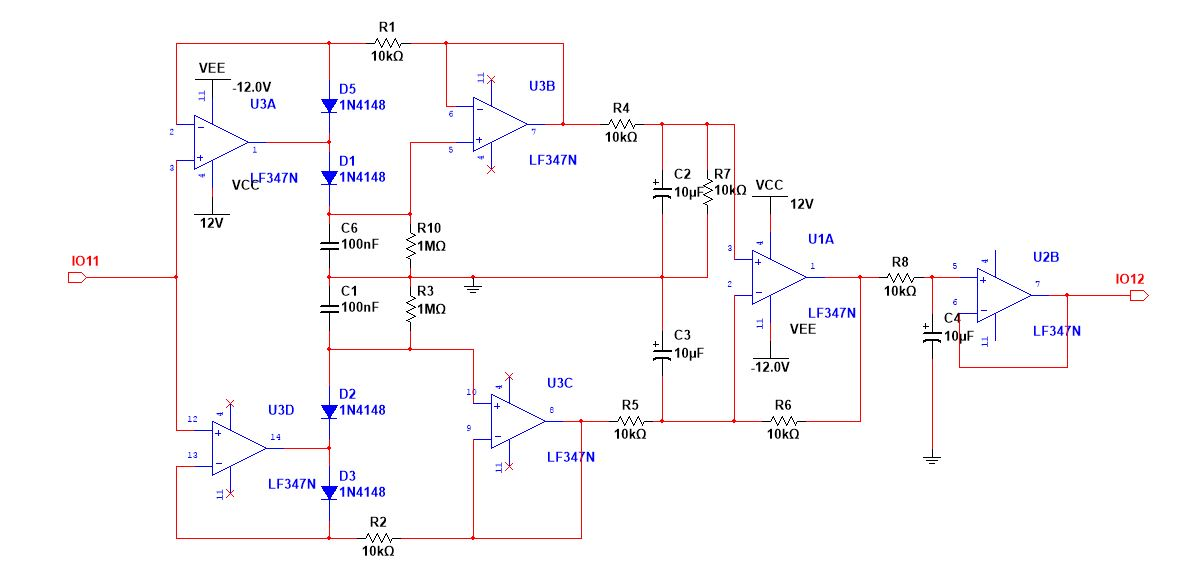
\includegraphics[width=\columnwidth]{PP.jpg}
\caption{峰值提取电路}\label{PP}
\end{figure}
\subsection{电压转换部分}
这部分输入一个稳定的正电压,输出一个频率稳定的方波,具体的电路如图\ref{VF}所示
\begin{figure}[H]
\centering
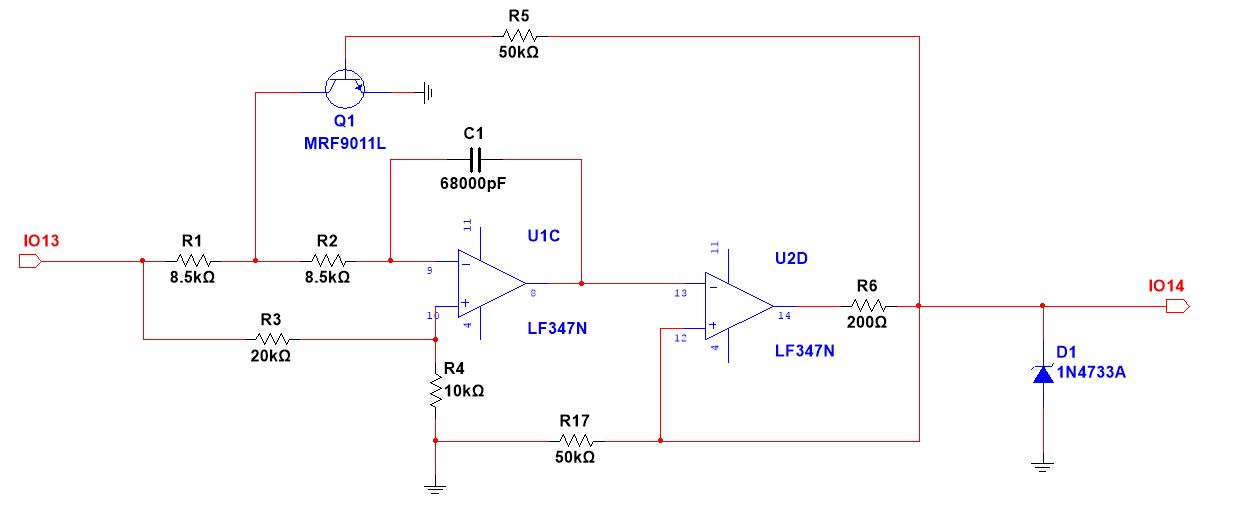
\includegraphics[width=\columnwidth]{VF.jpg}
\caption{压频转换电路}
\label{VF}
\end{figure}

\noindent 这个电路参考了模拟电子技术基础书上的压频转换电路的设计,具体原理略去。经过简单计算可以得到,电路在输入电压的控制下可以约为输出$50U_I\mathrm{Hz/V}$频率的方波,经过稳压之后输出共后级电路处理。

\noindent 电路涉及的电阻较多,因此受到电阻型号和相对误差的影响,电路的具体的参数(如选择的电阻电容)选择在电路搭建的过程中也需要进一步的选取,这里的仿真就先略去。
\subsection{FPGA部分}
\begin {wrapfigure}{r}{0pt}
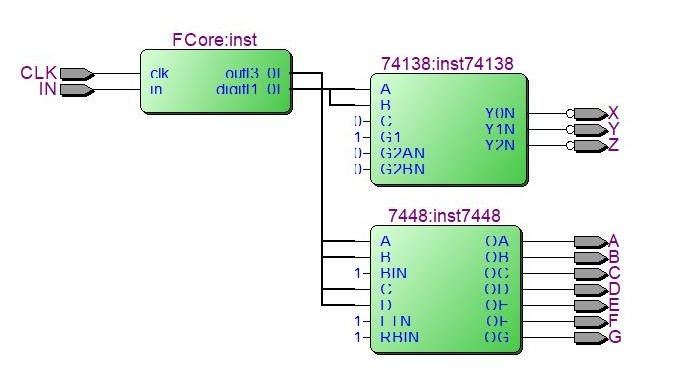
\includegraphics [width=30mm]{Block.jpg}
\caption{频率计数电路布置}
\label{DA}
\end {wrapfigure}
这部分要求将模拟电路输出的方波信号计数,得到最后要求显示的频率,为数字电路部分,电路模块图如图\ref{DA}所示。其中FCore模块是核心模块,负责在FPGA上的50MHz时钟下输出输入波形in的频率并在数码管中扫描显示。选通端由74138确定,数码管由7448驱动。

\noindent FCore模块的具体实现由Verilog代码给出。模块首先将输入时钟分频为1Hz,并在1Hz时钟上升沿设置输出记号。在输入in的每个上升沿,模块进行十进制计数。如果此时发现设置了输出记号,则清除此记号之后将当前值输出显示清零。

\noindent FCore也同时满足了一些诸如扫描数码管的功能,具体见下面的代码

\noindent \noindent
\ttfamily
\hlstd{}\hllin{01\ }\hlkwa{module\ }\hlstd{}\hlkwd{FCore\ }\hlstd{}\hlopt{(}\hlstd{clk}\hlopt{,}\hlstd{in}\hlopt{,}\hlstd{out}\hlopt{,}\hlstd{digit}\hlopt{);}\\
\hllin{02\ }\hlstd{}\hlkwa{input\ }\hlstd{clk}\hlopt{;}\\
\hllin{03\ }\hlstd{}\hlkwa{input\ }\hlstd{in}\hlopt{;}\\
\hllin{04\ }\hlstd{}\hlkwa{output\ }\hlstd{}\hlopt{{[}}\hlstd{}\hlnum{1}\hlstd{}\hlopt{:}\hlstd{}\hlnum{0}\hlstd{}\hlopt{{]}\ }\hlstd{digit}\hlopt{;}\\
\hllin{05\ }\hlstd{}\hlkwa{output\ }\hlstd{}\hlopt{{[}}\hlstd{}\hlnum{3}\hlstd{}\hlopt{:}\hlstd{}\hlnum{0}\hlstd{}\hlopt{{]}\ }\hlstd{out}\hlopt{;}\\
\hllin{06\ }\hlstd{}\hlkwa{reg\ }\hlstd{sec}\hlopt{;}\\
\hllin{07\ }\hlstd{}\hlkwa{reg\ }\hlstd{a\ }\hlopt{=\ }\hlstd{}\hlnum{0}\hlstd{}\hlopt{;}\\
\hllin{08\ }\hlstd{}\hlkwa{reg\ }\hlstd{b\ }\hlopt{=\ }\hlstd{}\hlnum{0}\hlstd{}\hlopt{;}\\
\hllin{09\ }\hlstd{}\hlkwa{reg\ }\hlstd{}\hlopt{{[}}\hlstd{}\hlnum{1}\hlstd{}\hlopt{:}\hlstd{}\hlnum{0}\hlstd{}\hlopt{{]}\ }\hlstd{digit\ }\hlopt{=\ }\hlstd{}\hlnum{2'b00}\hlstd{}\hlopt{;}\\
\hllin{10\ }\hlstd{}\hlkwa{reg\ }\hlstd{}\hlopt{{[}}\hlstd{}\hlnum{3}\hlstd{}\hlopt{:}\hlstd{}\hlnum{0}\hlstd{}\hlopt{{]}\ }\hlstd{out}\hlopt{;}\\
\hllin{11\ }\hlstd{}\hlkwa{reg\ }\hlstd{}\hlopt{{[}}\hlstd{}\hlnum{3}\hlstd{}\hlopt{:}\hlstd{}\hlnum{0}\hlstd{}\hlopt{{]}\ }\hlstd{num\ }\hlopt{{[}}\hlstd{}\hlnum{2}\hlstd{}\hlopt{:}\hlstd{}\hlnum{0}\hlstd{}\hlopt{{]};}\\
\hllin{12\ }\hlstd{}\hlkwa{reg\ }\hlstd{}\hlopt{{[}}\hlstd{}\hlnum{3}\hlstd{}\hlopt{:}\hlstd{}\hlnum{0}\hlstd{}\hlopt{{]}\ }\hlstd{\textunderscore num\ }\hlopt{{[}}\hlstd{}\hlnum{2}\hlstd{}\hlopt{:}\hlstd{}\hlnum{0}\hlstd{}\hlopt{{]};}\\
\hllin{13\ }\hlstd{}\hlkwa{reg\ }\hlstd{}\hlopt{{[}}\hlstd{}\hlnum{11}\hlstd{}\hlopt{:}\hlstd{}\hlnum{0}\hlstd{}\hlopt{{]}\ }\hlstd{div\ }\hlopt{=\ }\hlstd{}\hlnum{12'b1}\hlstd{}\hlopt{;}\\
\hllin{14\ }\hlstd{}\hlkwa{reg\ }\hlstd{}\hlopt{{[}}\hlstd{}\hlnum{27}\hlstd{}\hlopt{:}\hlstd{}\hlnum{0}\hlstd{}\hlopt{{]}\ }\hlstd{counter\ }\hlopt{=\ }\hlstd{}\hlnum{28'b0}\hlstd{}\hlopt{;}\\
\hllin{15\ }\hlstd{}\hlkwa{always\ }\hlstd{}\hlopt{@\ (}\hlstd{}\hlkwa{posedge\ }\hlstd{clk}\hlopt{)}\\
\hllin{16\ }\hlstd{}\hlkwa{begin}\\
\hllin{17\ }\hlstd{}\hlslc{//TODO:\ div\ the\ 50MHz\ clock\ to\ 1Hz}\\
\hllin{18\ }\hlstd{\ }\hlkwa{if}\hlstd{}\hlopt{(}\hlstd{counter\ }\hlopt{==\ }\hlstd{}\hlnum{28'd25000000}\hlstd{}\hlopt{)}\\
\hllin{19\ }\hlstd{\ }\hlkwa{begin}\\
\hllin{20\ }\hlstd{}\hlstd{\ \ }\hlstd{sec\ }\hlopt{$<$=\ $\sim$}\hlstd{sec}\hlopt{;}\\
\hllin{21\ }\hlstd{}\hlstd{\ \ }\hlstd{counter\ }\hlopt{=\ }\hlstd{}\hlnum{28'b1}\hlstd{}\hlopt{;}\\
\hllin{22\ }\hlstd{\ }\hlkwa{end}\\
\hllin{23\ }\hlstd{\ }\hlkwa{else\ }\\
\hllin{24\ }\hlstd{}\hlstd{\ \ }\hlstd{counter\ }\hlopt{$<$=\ }\hlstd{counter\ }\hlnum{+\ 1'b1}\hlstd{}\hlopt{;}\\
\hllin{25\ }\hlstd{}\hlstd{\ \ }\hlstd{\\
\hllin{26\ }\ }\hlslc{//TODO:\ div\ a\ sweeping\ signal}\\
\hllin{27\ }\hlstd{\ }\hlkwa{if}\hlstd{}\hlopt{(}\hlstd{div\ }\hlopt{==\ }\hlstd{}\hlnum{28'b0}\hlstd{}\hlopt{)}\\
\hllin{28\ }\hlstd{\ }\hlkwa{begin}\\
\hllin{29\ }\hlstd{}\hlstd{\ \ }\hlstd{div\ }\hlopt{$<$=\ }\hlstd{div\ }\hlnum{+\ 1'b1}\hlstd{}\hlopt{;}\\
\hllin{30\ }\hlstd{}\hlstd{\ \ }\hlstd{}\hlkwa{if}\hlstd{}\hlopt{(}\hlstd{digit\ }\hlopt{==\ }\hlstd{}\hlnum{2'b10}\hlstd{}\hlopt{)}\\
\hllin{31\ }\hlstd{}\hlstd{\ \ \ }\hlstd{digit\ }\hlopt{$<$=\ }\hlstd{}\hlnum{2'b00}\hlstd{}\hlopt{;}\\
\hllin{32\ }\hlstd{}\hlstd{\ \ }\hlstd{}\hlkwa{else}\\
\hllin{33\ }\hlstd{}\hlstd{\ \ \ }\hlstd{digit\ }\hlopt{$<$=\ }\hlstd{digit\ }\hlnum{+\ 1'b1}\hlstd{}\hlopt{;}\\
\hllin{34\ }\hlstd{\ }\hlkwa{end}\\
\hllin{35\ }\hlstd{\ }\hlkwa{else\ }\\
\hllin{36\ }\hlstd{}\hlstd{\ \ }\hlstd{div\ }\hlopt{$<$=\ }\hlstd{div\ }\hlnum{+\ 1'b1}\hlstd{}\hlopt{;}\\
\hllin{37\ }\hlstd{}\hlstd{\ \ }\hlstd{\\
\hllin{38\ }\ }\hlkwa{if}\hlstd{}\hlopt{(}\hlstd{div\ }\hlopt{==\ }\hlstd{}\hlnum{28'd10}\hlstd{}\hlopt{)}\\
\hllin{39\ }\hlstd{}\hlstd{\ \ }\hlstd{out\ }\hlopt{$<$=\ }\hlstd{num}\hlopt{{[}}\hlstd{digit}\hlopt{{]};}\\
\hllin{40\ }\hlstd{}\hlkwa{end}\\
\hllin{41\ }\hlstd{}\\
\hllin{42\ }\hlkwa{always\ }\hlstd{}\hlopt{@\ (}\hlstd{}\hlkwa{posedge\ }\hlstd{sec}\hlopt{)}\\
\hllin{43\ }\hlstd{}\hlkwa{begin}\\
\hllin{44\ }\hlstd{}\hlslc{//TODO:\ clear\ the\ output\ }\\
\hllin{45\ }\hlstd{a\ }\hlopt{$<$=\ $\sim$}\hlstd{b}\hlopt{;}\\
\hllin{46\ }\hlstd{}\hlkwa{end}\\
\hllin{47\ }\hlstd{}\\
\hllin{48\ }\hlkwa{always\ }\hlstd{}\hlopt{@\ (}\hlstd{}\hlkwa{posedge\ }\hlstd{in}\hlopt{)}\\
\hllin{49\ }\hlstd{}\hlkwa{begin}\\
\hllin{50\ }\hlstd{}\hlslc{//TODO:\ count}\\
\hllin{51\ }\hlstd{\ }\hlkwa{if}\hlstd{}\hlopt{(}\hlstd{a\ }\hlopt{==\ }\hlstd{b}\hlopt{)}\\
\hllin{52\ }\hlstd{\ }\hlkwa{begin}\\
\hllin{53\ }\hlstd{}\hlstd{\ \ }\hlstd{}\hlkwa{if}\hlstd{}\hlopt{(}\hlstd{\textunderscore num}\hlopt{{[}}\hlstd{}\hlnum{0}\hlstd{}\hlopt{{]}\ $<$\ }\hlstd{}\hlnum{4'd9}\hlstd{}\hlopt{)}\\
\hllin{54\ }\hlstd{}\hlstd{\ \ \ }\hlstd{\textunderscore num}\hlopt{{[}}\hlstd{}\hlnum{0}\hlstd{}\hlopt{{]}\ $<$=\ }\hlstd{\textunderscore num}\hlopt{{[}}\hlstd{}\hlnum{0}\hlstd{}\hlopt{{]}\ }\hlstd{}\hlnum{+\ 4'b0001}\hlstd{}\hlopt{;}\\
\hllin{55\ }\hlstd{}\hlstd{\ \ }\hlstd{}\hlkwa{else}\\
\hllin{56\ }\hlstd{}\hlstd{\ \ }\hlstd{}\hlkwa{begin}\\
\hllin{57\ }\hlstd{}\hlstd{\ \ \ }\hlstd{}\hlkwa{if}\hlstd{}\hlopt{(}\hlstd{\textunderscore num}\hlopt{{[}}\hlstd{}\hlnum{1}\hlstd{}\hlopt{{]}\ $<$\ }\hlstd{}\hlnum{4'd9}\hlstd{}\hlopt{)}\\
\hllin{58\ }\hlstd{}\hlstd{\ \ \ }\hlstd{}\hlkwa{begin\ }\\
\hllin{59\ }\hlstd{}\hlstd{\ \ \ \ }\hlstd{\textunderscore num}\hlopt{{[}}\hlstd{}\hlnum{1}\hlstd{}\hlopt{{]}\ $<$=\ }\hlstd{\textunderscore num}\hlopt{{[}}\hlstd{}\hlnum{1}\hlstd{}\hlopt{{]}\ }\hlstd{}\hlnum{+\ 4'b0001}\hlstd{}\hlopt{;}\\
\hllin{60\ }\hlstd{}\hlstd{\ \ \ \ }\hlstd{\textunderscore num}\hlopt{{[}}\hlstd{}\hlnum{0}\hlstd{}\hlopt{{]}\ $<$=\ }\hlstd{}\hlnum{4'b0000}\hlstd{}\hlopt{;}\\
\hllin{61\ }\hlstd{}\hlstd{\ \ \ }\hlstd{}\hlkwa{end}\\
\hllin{62\ }\hlstd{}\hlstd{\ \ \ }\hlstd{}\hlkwa{else}\\
\hllin{63\ }\hlstd{}\hlstd{\ \ \ }\hlstd{}\hlkwa{begin}\\
\hllin{64\ }\hlstd{}\hlstd{\ \ \ \ }\hlstd{\textunderscore num}\hlopt{{[}}\hlstd{}\hlnum{0}\hlstd{}\hlopt{{]}\ $<$=\ }\hlstd{}\hlnum{4'b0000}\hlstd{}\hlopt{;}\\
\hllin{65\ }\hlstd{}\hlstd{\ \ \ \ }\hlstd{\textunderscore num}\hlopt{{[}}\hlstd{}\hlnum{1}\hlstd{}\hlopt{{]}\ $<$=\ }\hlstd{}\hlnum{4'b0000}\hlstd{}\hlopt{;}\\
\hllin{66\ }\hlstd{}\hlstd{\ \ \ \ }\hlstd{\textunderscore num}\hlopt{{[}}\hlstd{}\hlnum{2}\hlstd{}\hlopt{{]}\ $<$=\ }\hlstd{\textunderscore num}\hlopt{{[}}\hlstd{}\hlnum{2}\hlstd{}\hlopt{{]}\ }\hlstd{}\hlnum{+\ 4'b0001}\hlstd{}\hlopt{;}\\
\hllin{67\ }\hlstd{}\hlstd{\ \ \ }\hlstd{}\hlkwa{end}\\
\hllin{68\ }\hlstd{}\hlstd{\ \ }\hlstd{}\hlkwa{end}\\
\hllin{69\ }\hlstd{\ }\hlkwa{end}\\
\hllin{70\ }\hlstd{\ }\hlkwa{else}\\
\hllin{71\ }\hlstd{\ }\hlkwa{begin}\\
\hllin{72\ }\hlstd{}\hlstd{\ \ }\hlstd{b\ }\hlopt{$<$=\ }\hlstd{a}\hlopt{;}\\
\hllin{73\ }\hlstd{}\hlstd{\ \ }\hlstd{num}\hlopt{{[}}\hlstd{}\hlnum{0}\hlstd{}\hlopt{{]}\ $<$=\ }\hlstd{\textunderscore num}\hlopt{{[}}\hlstd{}\hlnum{0}\hlstd{}\hlopt{{]};}\\
\hllin{74\ }\hlstd{}\hlstd{\ \ }\hlstd{num}\hlopt{{[}}\hlstd{}\hlnum{1}\hlstd{}\hlopt{{]}\ $<$=\ }\hlstd{\textunderscore num}\hlopt{{[}}\hlstd{}\hlnum{1}\hlstd{}\hlopt{{]};}\\
\hllin{75\ }\hlstd{}\hlstd{\ \ }\hlstd{num}\hlopt{{[}}\hlstd{}\hlnum{2}\hlstd{}\hlopt{{]}\ $<$=\ }\hlstd{\textunderscore num}\hlopt{{[}}\hlstd{}\hlnum{2}\hlstd{}\hlopt{{]};}\\
\hllin{76\ }\hlstd{}\hlstd{\ \ }\hlstd{\textunderscore num}\hlopt{{[}}\hlstd{}\hlnum{0}\hlstd{}\hlopt{{]}\ $<$=\ }\hlstd{}\hlnum{4'b0001}\hlstd{}\hlopt{;}\\
\hllin{77\ }\hlstd{}\hlstd{\ \ }\hlstd{\textunderscore num}\hlopt{{[}}\hlstd{}\hlnum{1}\hlstd{}\hlopt{{]}\ $<$=\ }\hlstd{}\hlnum{4'b0000}\hlstd{}\hlopt{;}\\
\hllin{78\ }\hlstd{}\hlstd{\ \ }\hlstd{\textunderscore num}\hlopt{{[}}\hlstd{}\hlnum{2}\hlstd{}\hlopt{{]}\ $<$=\ }\hlstd{}\hlnum{4'b0000}\hlstd{}\hlopt{;}\\
\hllin{79\ }\hlstd{\ }\hlkwa{end}\\
\hllin{80\ }\hlstd{}\hlkwa{end}\\
\hllin{81\ }\hlstd{}\hlkwa{endmodule}\hlstd{}\\
\mbox{}
\normalfont
\normalsize

\section{电路工作原理说明}\small
\subsection{峰峰值提取部分}
\begin {wrapfigure}{r}{0pt}
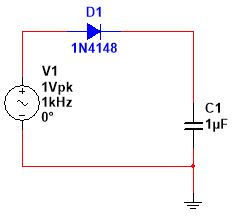
\includegraphics [width=30mm]{f1.jpg}
\caption{基本峰值提取电路}
\label{f1}
\end {wrapfigure}
 由于采取了和老师给出的电路不同的设计,因此这里重新将模拟部分的两个电路的工作原理详细说明如下。

\subsubsection{简单峰值提取电路}

\noindent 如图\ref{f1}所示
是简单峰值提取电路,我们首先先认为二极管导通压降为0,
则若输入电压大于电容C上的电压,电容充电升压,如果输入电压小于
电容C上的电压,电容不放电,因此电容上保持的是整个电路的历史最高输入电压。

\noindent 然而实际电路中,由于存在二极管分压,输出的电压值显然和最大峰值相差二极管导通电压。需要采用其他的电路来改进这个电路

\subsubsection{精密峰值提取电路}

\begin {wrapfigure}{r}{0pt}
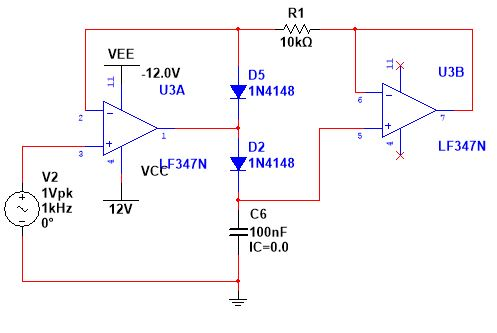
\includegraphics [width=30mm]{f2.jpg}
\caption{精密峰值提取电路}
\label{f2}
\end {wrapfigure}
如图\ref{f2}所示,首先分析二极管D5能否导通,如果D5能导通,则运放U3A工作在负反馈状态,而如果D5截断,运放U3A处于比较器状态。我们假设D5导通,则可以看出运放U3A输出电压为$V_2-V_{PN}$,电容C6随运放U3B跟随,此时可以明显分析出此时C6上电压大于输入电压,因此此时C6电压保持不变,条件为$V_2<U_{C6}$

\noindent 当输入电压大于电容上电压时,上述推理不成立,运放工作在非线性区。可以看出,此时U3A上有$U_P=V_2,U_N=V{C6}$,运放输出正摆幅,对C6高速充电(因为输入电压很大而电阻很小)保证电路响应顺畅。

\noindent 因此在当前环境下U3B阻抗变换之后可以输出质量相当好的输入电压峰值。

\subsubsection{其他辅助设计}
\begin{itemize}
\item 峰值电容放电回路

\noindent 上述设计能够准确检测出输入电压的历史最大值,但如果使用者希望动态测量峰峰值的话,当输入电压峰值减小之后整个电路将被锁死不工作。因此在C上并联放电电阻R使得当输入减小之后C能够缓慢放电最后达到测量目的。当输入电压峰值稳定时,由于不断有周期性峰值的影响,整个电路整体稳定,但略有纹波。

\item 双向峰峰值检测电路

\noindent 将上述设计反向,得到负峰值检测电路,整个前级电路的如图\ref{f3}所示。

\end{itemize}

\begin{figure}[H]
\centering
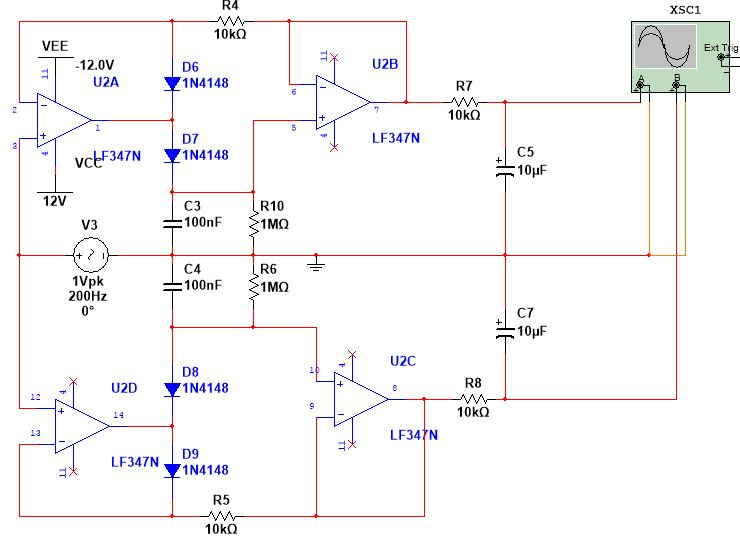
\includegraphics[width=\columnwidth]{f3.jpg}
\caption{双向峰峰值检测电路}
\label{f3}
\end{figure}

\subsubsection{综合输出}
\noindent 最后利用减法器将正峰值和负峰值相减,得到峰峰值。同时在电路上引入适当的一节低通滤波电路消除之前由于RC环节引入的纹波,整个电路如图\ref{PP}所示。在$V_{PP}=5\mathrm{V},f=20\mathrm{Hz}$的作用下输出的波形如图\ref{f4}所示。

\noindent 可以看出,经过0.6s的过渡时间之后,电路输出电压已经很稳定了,而且由于采用负反馈运放,输出电压的稳定性也特别理想。
\begin{figure}[H]
\centering
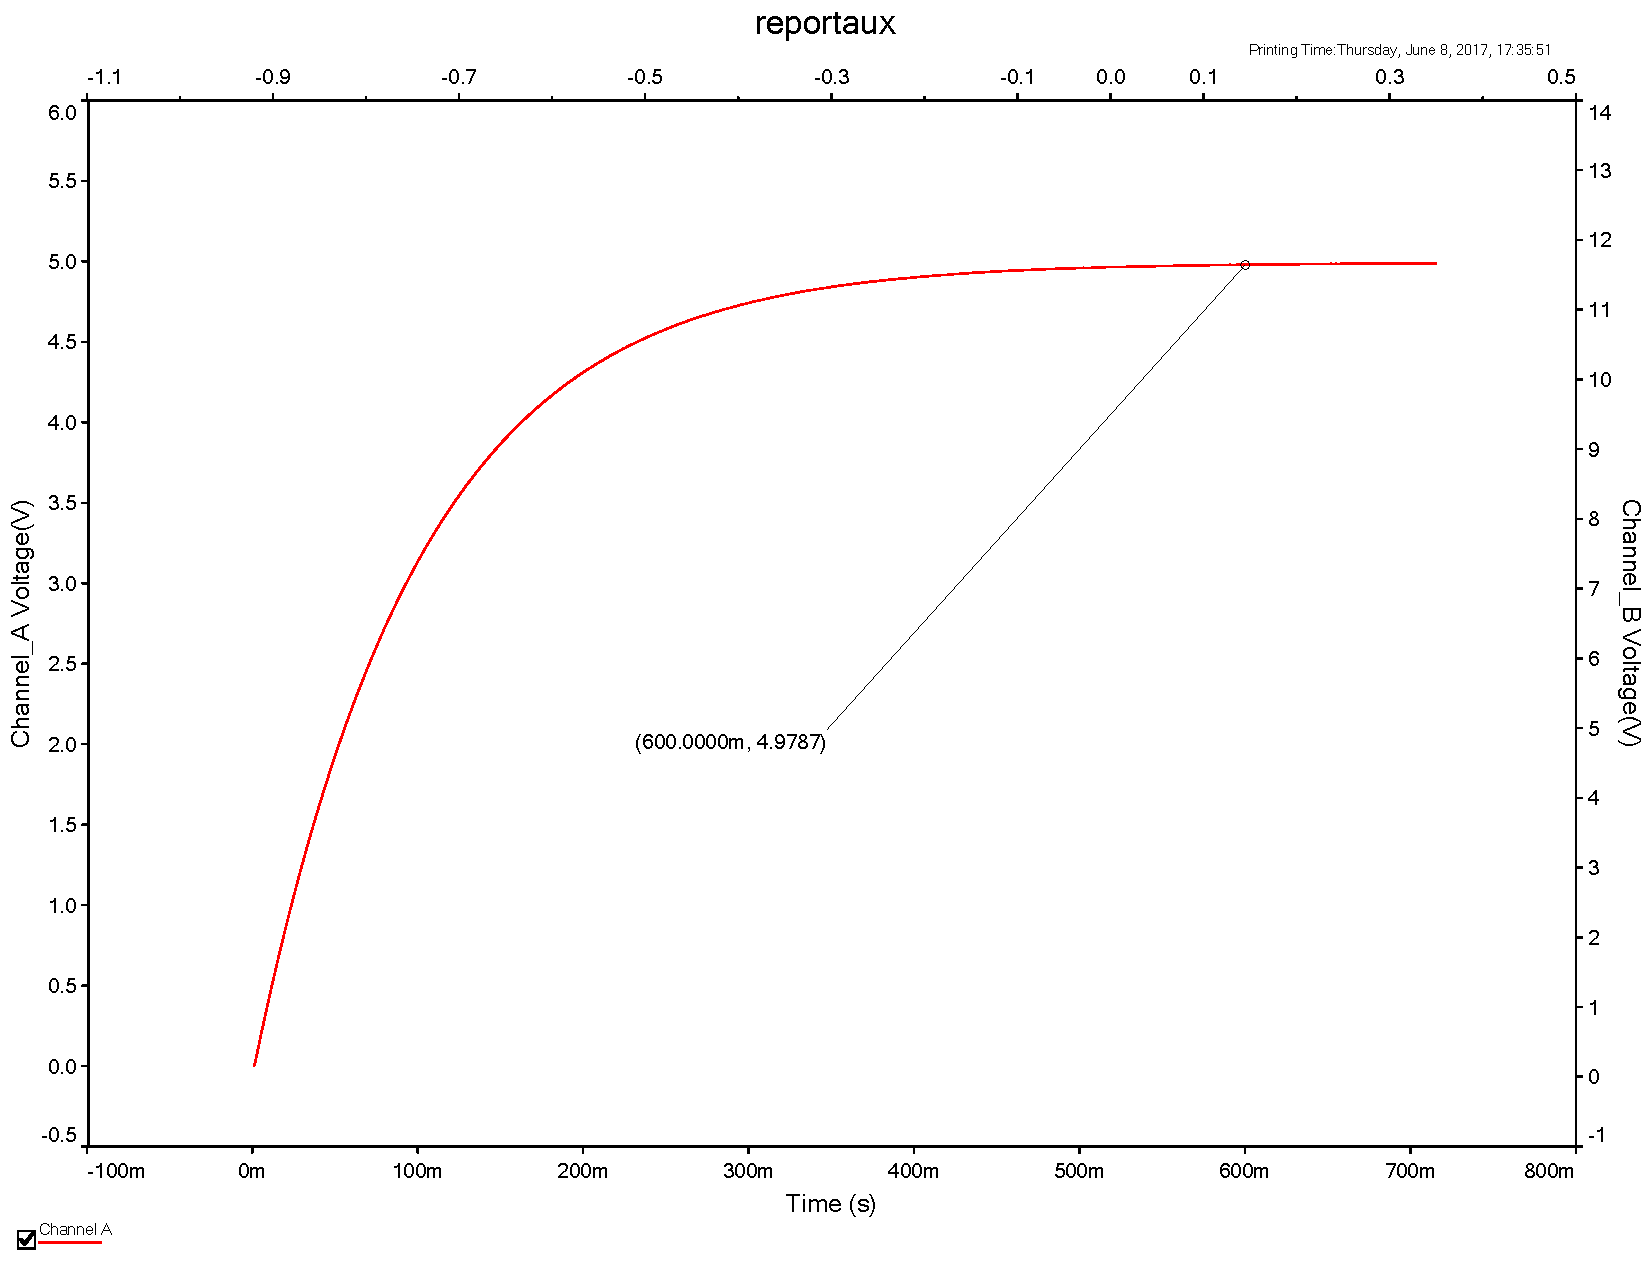
\includegraphics[width=\columnwidth]{f4.pdf}
\caption{峰峰值检测电路输出波形}
\label{f4}
\end{figure}

\subsection{V-F转换部分}
\noindent 参考模拟电子技术基础的习题7.24搭建了基于运放的复位式压控振荡电路,如图\ref{f5}所示。

\subsubsection{工作原理}
\noindent 复位式压控振荡电路主要由滞回比较器、积分器及电子开关组成:运放A2与R2,R3以及稳压管D1,D2构成滞回比较器,运放A1与电容C及输入端电阻构成积分器,晶体管Q1及电阻R5构成电子开关。

\noindent 当运放A2输出高电平时,晶体管饱和导通,视为开关接地,电容C充电,直到运放A1输出端$u_{o1}$达到阈值电压$+U_T$使得A2输出低电平。当A2输出低电平,晶体管截止,电容C反向充电,直到运放A1输出端$u_{o1}$达到阈值电压$-U_T$使得A2输出高电平,进入下一个循环。
\begin{figure}[H]
\centering
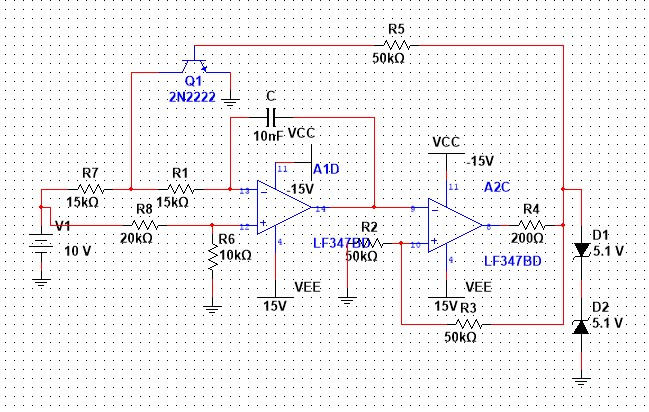
\includegraphics[width=\columnwidth]{f5.jpg}
\caption{VF变换电路图}
\label{f5}
\end{figure}

\subsubsection{定量分析}
\noindent 当晶体管导通时
$i_c=\frac{0-u_N1}{3R1}=-\frac{u_I}{3R1}$
当晶体管截止时
$u_{o1} = u_{o1}(t_0)+\frac{u_I}{3R_1C}(t_1-t_0)$
另外,滞回比较器阈值电压
$\begin{cases}
i_c = \frac{u_I}{3R_1}\\
u_{o1} = u_{o1}(t_1)-\frac{u_I}{3R_1C}(t_2-t_1)
\end{cases}$
则可以得到振荡频率
\noindent $f=\frac{1}{T}=\frac{u_I}{12R_1CU_T}$
振荡频率与输入电压呈线性

\noindent 设计中要求前级输入电压$U_I$和输出信号频率$f$的关系为$f = 100 U_I \mathrm{Hz/V}$因此设计电路参数图中C改为20nF其他参数不变。

\noindent 仿真得到输入1V波形如图\ref{f6}所示,测得频率接近100Hz,效果还是比较理想的,同时方波波形稳定,可以提供给下级FPGA工作,剩余误差可以在实验过程中微调解决。不是设计问题。

\begin{figure}[H]
\centering
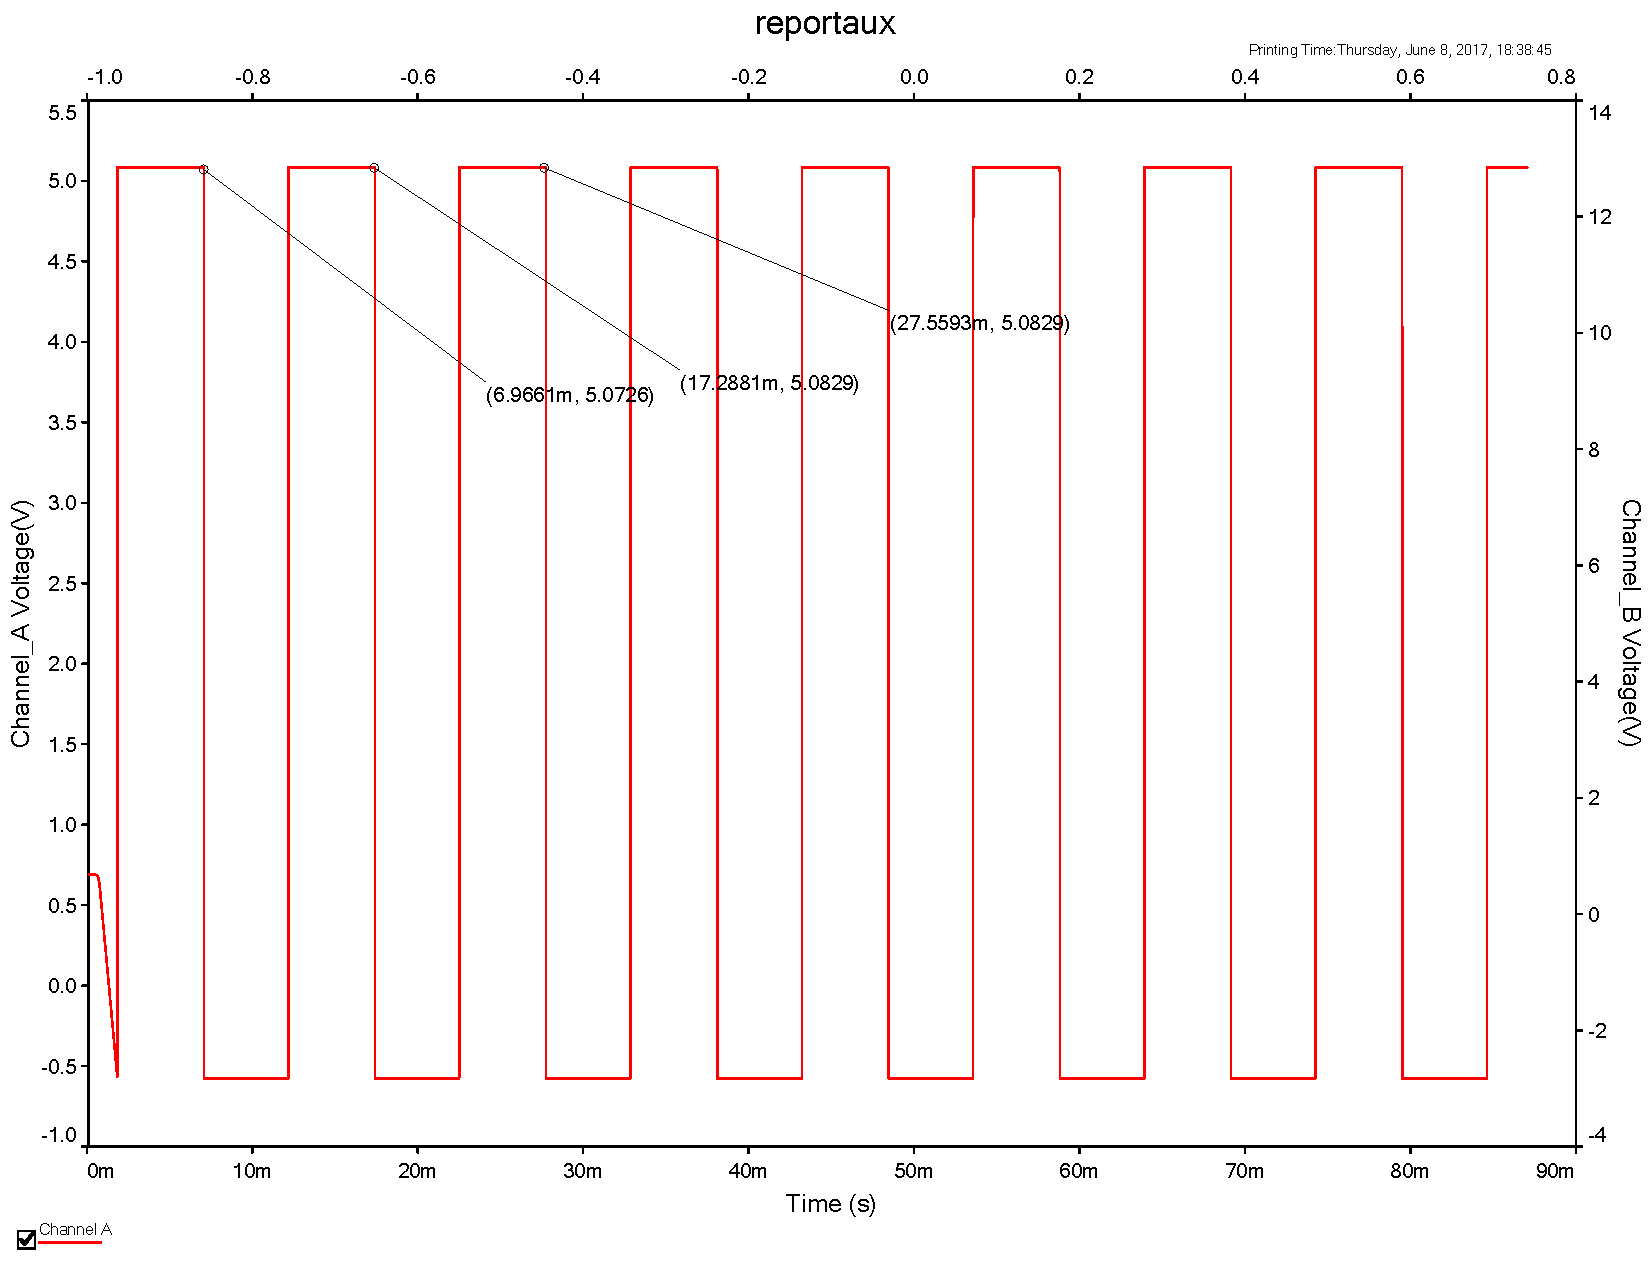
\includegraphics[width=\columnwidth]{f6.pdf}
\caption{VF输出波形}
\label{f6}
\end{figure}

\section{实验结果}\small
\noindent 对实际电路进行测试的得到了如表\ref{t1}的结果,可以看出电路输出的电压值(在FPGA上显示得到)的精度相当高。

\section{总结}\small
\noindent 本次实验自己新设计了电路,相比于老师提供的电路,除了输出准确之外,还能够在一定程度上接受输入电压的直流偏置和各种波形(因为前级电路峰值提取不受波形的影响)

\noindent 另外,这次实验在12周提前两周就已经完成了电路的搭建并利用myDac完成了初步的测试工作。由于电路搭建和FPGA的设计是一起考虑的,体现了设计的整体性和模块之间的相互兼容的特性,如方波占空比适中,边沿锋利使得FPGA可以高精度工作等。可以说,这次实验是相当成功的。
\begin{table}[H]
\centering
\caption{实验结果}
\label{t1}
\begin{sideways}
\begin{tabular}{|c|c|c|c|c|c|c|c|c|}
\hline
$V_{I}$ & 20Hz & 200Hz&$V_{I}$ & 20Hz & 200Hz&$V_{I}$ & 20Hz & 200Hz\\ \hline
5 & 4.95 & 4.98 & 0.9 & 0.89 & 0.90 &0.4 & 0.39 & 0.40\\ \hline
4 & 3.95 & 3.98 & 0.8 & 0.79 & 0.78 &0.3 & 0.29 & 0.30\\ \hline
3 & 2.96 & 2.98 & 0.7 & 0.69 & 0.68 & 0.2 & 0.19 & 0.19 \\ \hline
2 & 1.97 & 1.98 & 0.6 & 0.59 & 0.59 & 0.1 & 0.10 & 0.10\\ \hline
1 & 0.98 & 0.99 & 0.5 & 0.50 & 0.49 &0.0 & 0.01 & 0.01\\ \hline
\end{tabular}
%
\end{sideways}
\end{table}
\end{multicols}
\end{document}